\documentclass[a4paper,11pt]{article}

%-------------------------
% Packages
%-------------------------
\usepackage{latexsym}
\usepackage[empty]{fullpage}
\usepackage{titlesec}
\usepackage[usenames,dvipsnames]{color}
\usepackage{verbatim}
\usepackage{enumitem}
\usepackage[hidelinks]{hyperref}
\usepackage{fancyhdr}
\usepackage{tabularx}
\usepackage{graphicx}
\usepackage{geometry}
\usepackage[T1]{fontenc}
\usepackage{lmodern}

%-------------------------
% Formatting & Margins
%-------------------------
\geometry{left=1.5cm, top=1.5cm, right=1.5cm, bottom=1.5cm}
\setlength{\footskip}{4.1pt}

\pagestyle{fancy}
\fancyhf{}
\fancyfoot{}
\renewcommand{\headrulewidth}{0pt}
\renewcommand{\footrulewidth}{0pt}

\urlstyle{same}

\raggedbottom
\raggedright
\setlength{\tabcolsep}{0in}

%-------------------------
% Custom Commands
%-------------------------
\titleformat{\section}{
  \vspace{-4pt}\scshape\raggedright\large\bfseries
}{}{0em}{}[\color{black}\titlerule \vspace{-5pt}]

\newcommand{\resumeItem}[1]{
  \item\small{{#1 \vspace{-2pt}}}
}

\newcommand{\resumeSubheading}[4]{
  \vspace{-2pt}\item
    \begin{tabular*}{0.97\textwidth}[t]{l@{\extracolsep{\fill}}r}
      \textbf{#1} & #2 \\
      \textit{\small#3} & \textit{\small #4} \\
    \end{tabular*}\vspace{-7pt}
}

\newcommand{\resumeProjectHeading}[2]{
    \item
    \begin{tabular*}{0.97\textwidth}{l@{\extracolsep{\fill}}r}
      \small#1 & #2 \\
    \end{tabular*}\vspace{-7pt}
}

\newcommand{\resumeSubHeadingListStart}{\begin{itemize}[leftmargin=0.15in, label={}]}
\newcommand{\resumeSubHeadingListEnd}{\end{itemize}}
\newcommand{\resumeItemListStart}{\begin{itemize}}
\newcommand{\resumeItemListEnd}{\end{itemize}\vspace{-5pt}}

%-------------------------
% CV STARTS HERE
%-------------------------
\begin{document}

%-------------------------
% Header
%-------------------------
\begin{tabular*}{\textwidth}{@{} l @{\extracolsep{\fill}} r @{}}
  \begin{minipage}[c]{0.68\textwidth}
    \textbf{\Huge Aakash Khadka} \\[4pt]
    \textbf{\large Data Engineer / Software Engineer} \\[4pt]
    \small
    \href{mailto:aakaskhadka@gmail.com}{aakaskhadka@gmail.com} \quad
    +49 155 6300 7796 \\[2pt]
    \href{https://www.linkedin.com/in/aakash-khadka-675b4a158/}{linkedin.com/in/aakash-khadka} \quad
    \href{https://github.com/Aakash7khadka}{github.com/Aakash7khadka} \\[2pt]
    Magdeburg, Germany
  \end{minipage}
  &
  \begin{minipage}[c]{0.25\textwidth}
    \raggedleft
    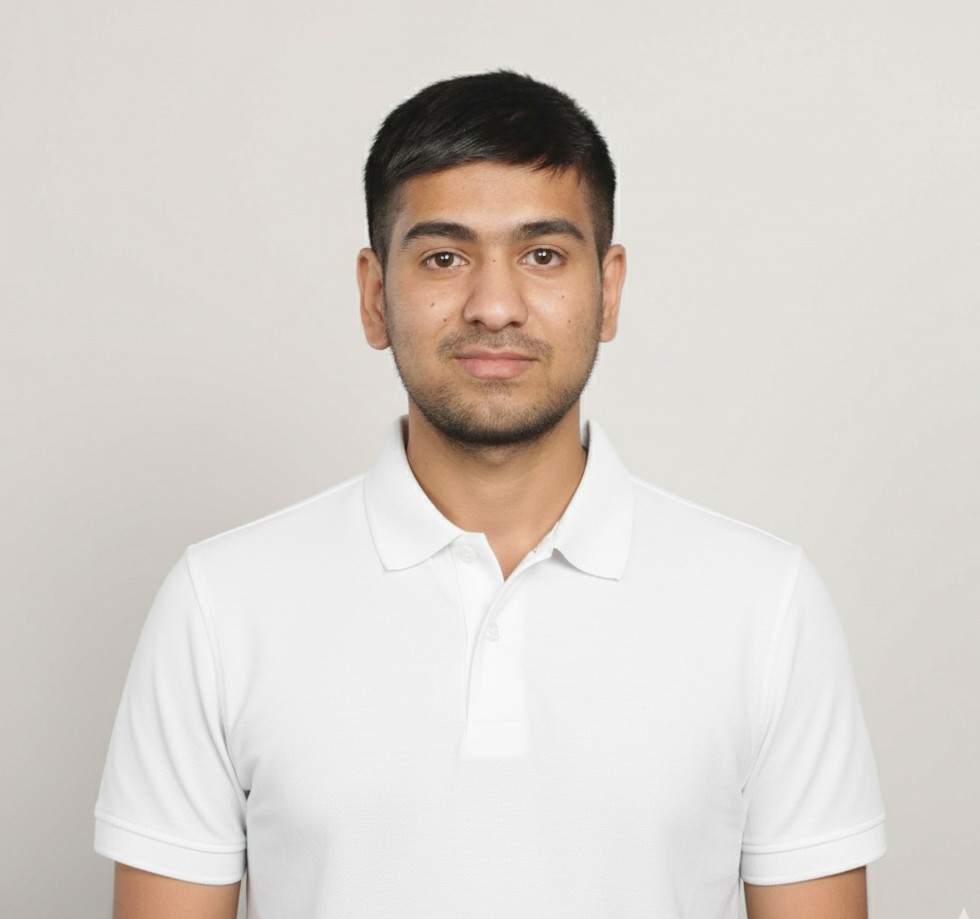
\includegraphics[width=3.2cm,height=3.2cm,keepaspectratio]{1.jpg}%
  \end{minipage}
\end{tabular*}

\vspace{6pt}

%-------------------------
% Profile
%-------------------------
\section{Profile}
 \begin{itemize}[leftmargin=0.15in, label={}]
    \small{\item{
     Data Engineer / Software Engineer with 2.5 years of professional experience building Big Data pipelines
     involving Hadoop/Spark batch processing at scale, Elasticsearch indexing, Java and Python module
     development for pipeline orchestration and processing, and real-time data anomaly detection in the
     index with AWS Lambda.
     Currently pursuing M.Sc.\ (Masters) in Data \& Knowledge Engineering at
     Otto-von-Guericke-Universitat Magdeburg (current grade: 1.7).
    }}
 \end{itemize}

%-------------------------
% Experience
%-------------------------
\section{Experience}
  \resumeSubHeadingListStart

    \resumeSubheading
      {Otto-von-Guericke-Universitat Magdeburg}{Magdeburg, Germany}
      {Research Assistant - RAG System Development}{12/2025 - Present}
      \resumeItemListStart
        \resumeItem{Developing a privacy-aware RAG chatbot using \textbf{Python}, \textbf{LangChain}, and vector databases for secure document retrieval and LLM integration.}
      \resumeItemListEnd

    \resumeSubheading
      {Otto-von-Guericke-Universitat Magdeburg}{Magdeburg, Germany}
      {Teaching Assistant - Information Retrieval}{10/2025 - 01/2026}
      \resumeItemListStart
        \resumeItem{Conducting weekly exercise sessions for 20+ students on indexing and ranking algorithms for information retrieval.}
        \resumeItem{Grading assignments and giving feedback as well as support on Projects.}
      \resumeItemListEnd

    \resumeSubheading
      {CedarGate Technologies}{Lalitpur, Nepal}
      {Software Engineer}{05/2022 - 09/2024}
      \resumeItemListStart
        \resumeItem{\textbf{Module Development:} Developed 20+ Java and Python data engineering modules covering ingestion, transformation, and orchestration to extend Big Data pipeline capabilities.}
        \resumeItem{\textbf{Hadoop Optimization:} Optimized Hadoop and Spark batch pipelines by reducing reducer-side processing, optimizing joins, removing redundant operations, eliminating recurring failures.}
        \resumeItem{\textbf{Job Orchestration:} Implemented conditional submission for \textbf{Spark} and Hadoop jobs based on data availability, reducing compute time by 30 minutes to 2 hours per client per batch processing.}
        \resumeItem{\textbf{Serverless Architecture:} Built a serverless variance detection system using \textbf{AWS Lambda} and \textbf{Elasticsearch} to automate data integrity checks (e.g., row counts, claim amounts) before client delivery.}
        \resumeItem{\textbf{ML Integration:} Integrated ML models (including \textbf{MARA}) into production pipelines and stored historical risk scores as \textbf{Protobuf objects} in \textbf{AWS S3} to enable efficient retrieval and seamless schema evolution.}
        \resumeItem{\textbf{Healthcare Compliance:} Achieved \textbf{HEDIS 2024 (NCQA)} certification and integrated \textbf{ACO REACH} standards, ensuring 100\% compliance to healthcare effectiveness protocols.}
        \resumeItem{\textbf{Search Engine Engineering:} Engineered a "Multi-Field Group By" feature in \textbf{Elasticsearch} that utilizes cardinality scores to restrict high-variance field selection, enabling stable aggregations on datasets exceeding 10 million records.}
      \resumeItemListEnd

    \resumeSubheading
      {LIS Nepal}{Lalitpur, Nepal}
      {Software Engineering Intern}{11/2020 - 04/2021}
      \resumeItemListStart
        \resumeItem{Developed responsive frontend modules for a financial compliance reporting system using \textbf{React.js}, ensuring accurate data visualization for regulatory audits.}
        \resumeItem{Gained practical exposure to \textbf{ETL} workflows and data warehouse architecture, applying \textbf{SQL} best practices for data extraction and transformation.}
      \resumeItemListEnd

  \resumeSubHeadingListEnd

%-------------------------
% Education
%-------------------------
\section{Education}
  \resumeSubHeadingListStart
    \resumeSubheading
      {Otto-von-Guericke-Universitat Magdeburg}{Magdeburg, Germany}
      {M.Sc.\ Data and Knowledge Engineering (Grade: 1.7)}{10/2024 - Present}
    \resumeSubheading
      {Tribhuvan University}{Kathmandu, Nepal}
      {B.Sc.\ Computer Science and Information Technology (German equiv.\ Grade: 2.0)}{08/2017 - 12/2021}
  \resumeSubHeadingListEnd

%-------------------------
% Projects
%-------------------------
\section{Projects}
  \resumeSubHeadingListStart
    \resumeProjectHeading
      {\textbf{BioSignal Prediction for Breathing Training} \emph{(Flutter, Medical Telemetry, Data Analysis)}}{}

    \textbf{Version 1:}
    \resumeItemListStart
      \resumeItem{Built a Python-based desktop prototype for personalized breathing training that guides users along a sinusoidal breathing trajectory to progressively reach GLI (Global Lung Initiative) spirometry targets.}
      \resumeItem{Applied Exponential Moving Average (EMA) and Kalman filtering for respiratory signal processing to reduce noise and remove drift from spirometry data.}
      \resumeItem{Modeled breathing performance improvement using the Exponential Law of Practice to dynamically adapt training difficulty and target breathing levels.}
      \resumeItem{Designed the system to provide personalized breathing targets derived from GLI reference values for improved respiratory training outcomes.}
      \resumeItem{Research paper based on this system currently \textbf{under preparation for publication}.}
    \resumeItemListEnd

    \textbf{Version 2: Ongoing}
    \resumeItemListStart
      \resumeItem{Following clinical review of Version 1 with a pulmonologist, extending the system into a medical telemetry platform enabling remote monitoring between patients and doctors.}
      \resumeItem{Designing a feedback-driven breathing training system allowing physicians to monitor respiratory performance and adjust patient-specific breathing targets.}
      \resumeItem{Established collaboration with a pulmonologist to conduct real-world validation of the breathing training system with 30+ patients.}
      \resumeItem{Developing a Flutter-based telemetry interface to support real-time respiratory data transmission and clinician feedback.}
    \resumeItemListEnd

    \resumeProjectHeading
      {\textbf{LLM Summary-Based Document Classification} \emph{(Python, Ollama, Scikit-learn)}}{}
      \resumeItemListStart
        \resumeItem{Benchmarked classification accuracy of LLM-generated summaries vs.\ full-text documents using local Ollama models, achieving comparable F1 scores with 70\% reduced input size.}
        \resumeItem{Validated that LLM-generated summaries perform competitively in classification accuracy tasks with significantly reduced computational overhead.}
      \resumeItemListEnd

  \resumeSubHeadingListEnd

%-------------------------
% Technical Skills
%-------------------------
\section{Technical Skills}
 \begin{itemize}[leftmargin=0.15in, label={}]
    \small{\item{
     \textbf{Programming:} Python, Java, SQL, Bash \\
     \textbf{Big Data \& Cloud:} PySpark, Hadoop (MapReduce, HDFS), AWS (Lambda, EC2, S3, CloudWatch), Elasticsearch \\
     \textbf{Data Engineering:} ETL/ELT Pipelines, Batch Processing, Pipeline Orchestration, Data Modeling, Protobuf \\
     \textbf{Data Science \& ML:} Pandas, NumPy, Scikit-learn, PyTorch, LangChain, NLP, Machine Learning \\
     \textbf{Tools \& Infrastructure:} Docker, Git, Maven, PostgreSQL, CI/CD, Linux
    }}
 \end{itemize}

%-------------------------
% Awards
%-------------------------
\section{Awards \& Certificates}
 \begin{itemize}[leftmargin=0.15in, label={}]
    \small{\item{
     \textbf{Itonics Hackathon:} 2nd Place (team competition) \\
     \textbf{Deep Learning Specialization:} Coursera (Andrew Ng, deeplearning.ai)
    }}
 \end{itemize}

%-------------------------
% Languages
%-------------------------
\section{Languages}
 \begin{itemize}[leftmargin=0.15in, label={}]
    \small{\item{
     \textbf{English:} C1 (fluent, working language) \quad
     \textbf{German:} A2 (actively improving, targeting B1) \quad
     \textbf{Nepali:} Native
    }}
 \end{itemize}

\end{document}